\documentclass[tikz,border=5pt,multi=tikzpicture]{standalone}
\usepackage[UTF8]{ctex}
\usepackage{amsmath}
\usetikzlibrary{arrows.meta,calc}
\definecolor{ink}{HTML}{17365D}
\definecolor{field}{HTML}{287DA8}
\definecolor{force}{HTML}{C56B2A}
\tikzset{every node/.style={font=\small},vec/.style={-{Stealth[length=2mm]},thick},helper/.style={gray,dashed}}
\newcommand{\halfball}[2]{
  \begin{scope}
    \clip (-#1,0) arc (180:360:#1) arc (0:180:#1 and {#1*.30})--cycle;
    \shade[ball color=field!45] (0,0) circle (#1);
  \end{scope}
  \draw[field!80!black,thick] (-#1,0) arc (180:360:#1);
  \filldraw[force,fill=force!22,thick] (0,0) ellipse (#1 and {#1*.30});
  \filldraw[field,fill=field!12,thick] (0,0) ellipse (#2 and {#2*.30});
}
\begin{document}
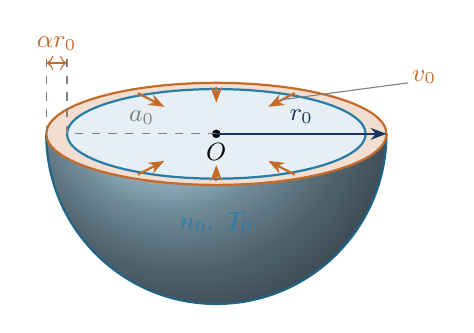
\begin{tikzpicture}[scale=1.2]
  \halfball{1.8}{1.58}
  \fill (0,0) circle (1.3pt) node[below] {$O$};
  \draw[vec,ink] (0,0)--(1.8,0) node[midway,above] {$r_0$};
  \draw[helper] (0,0)--(-1.58,0) node[midway,above] {$a_0$};
  \draw[<->,force] (-1.8,.75)--(-1.58,.75);
  \draw[helper] (-1.8,0)--(-1.8,.8);\draw[helper] (-1.58,0)--(-1.58,.8);
  \node[force,above] at (-1.69,.78) {$\alpha r_0$};
  \foreach \t in {60,90,120,240,270,300}{
    \draw[vec,force] ({1.66*cos(\t)},{.498*sin(\t)})--({1.1*cos(\t)},{.33*sin(\t)});
  }
  \node[field] at (0,-.95) {$n_0,\ T_0$};
  \node[force] at (2.2,.6) {$v_0$};
  \draw[gray] (2.03,.54)--(.68,.36);
\end{tikzpicture}
\begin{tikzpicture}
  \draw[helper] (-.4,-1.4) rectangle (8.3,1.4);
  \node[ink] at (1.1,.72) {向内壳层};
  \node[ink] at (1.1,.08) {$K_0=\tfrac12m_s v_0^2$};
  \node[ink] at (1.1,-.75) {$K_1=0$};
  \draw[vec,force] (2.9,0)--(4.15,0) node[midway,above] {$W$};
  \node[field] at (6.15,.72) {内部核心};
  \node[field] at (6.15,.08) {$\Delta U=\nu_c C_v(T_1-T_0)$};
  \node[field] at (6.15,-.75) {$Q=0$};
  \node at (3.95,-1.78) {系统边界包含壳层与核心};
\end{tikzpicture}
\begin{tikzpicture}
  \begin{scope}
    \halfball{1.55}{1.48}
    \draw[vec,ink] (0,0)--(1.48,0) node[midway,above] {$a_0$};
    \node[field] at (0,-.72) {$N_c,\ n_0,\ T_0$};
    \node at (0,-1.9) {压缩开始};
  \end{scope}
  \draw[vec,force] (2.1,-.6)--(3,-.6);
  \begin{scope}[xshift=4.7cm]
    \halfball{.92}{.85}
    \draw[vec,ink] (0,0)--(.85,0) node[midway,above] {$a_1$};
    \node[field] at (0,-1.27) {$N_c,\ n_1,\ T_1$};
    \node at (0,-1.9) {最大压缩};
  \end{scope}
\end{tikzpicture}
\begin{tikzpicture}[x=5.6cm,y=1.1cm]
  \fill[force!13] (.6,{1/.36})--plot[domain=.6:1,samples=80] (\x,{1/(\x*\x)})--(1,{1/.36})--cycle;
  \draw[vec,gray] (.5,0)--(1.09,0) node[right] {$a/a_0$};
  \draw[vec,gray] (.52,0)--(.52,3.18) node[above] {$U/U_0$};
  \draw[field,thick,domain=.58:1.02,samples=80] plot (\x,{1/(\x*\x)});
  \draw[force,thick] (.6,{1/.36})--(1.04,{1/.36}) node[right] {$U_0+K_0$};
  \draw[helper] (.6,0)--(.6,{1/.36});\draw[helper] (1,0)--(1,{1/.36});
  \fill[field] (.6,{1/.36}) circle (1.3pt);\fill[field] (1,1) circle (1.3pt);
  \node[below] at (.6,0) {$a_1/a_0$};\node[below] at (1,0) {$1$};
  \draw[<->,force] (.95,1.108)--(.95,{1/.36}) node[midway,left] {$K_s/U_0$};
  \node[field,right] at (.6,.65) {$U(a)/U_0$};
  \draw[vec,ink] (.93,-.58)--(.68,-.58) node[midway,below] {压缩方向};
\end{tikzpicture}
\end{document}
